\documentclass[11pt, a4paper]{article}
%-----------------------
%- 	PACKAGES & SETTINGS
%-----------------------
\usepackage[a4paper,top=2cm,bottom=2cm,left=2cm,right=2cm]{geometry}
\renewcommand{\baselinestretch}{1} 
\usepackage[utf8]{inputenc}
\usepackage[T1]{fontenc}
\usepackage[italian]{babel}
\usepackage{xcolor}
\usepackage{tabto}
\usepackage{hyperref}
\hypersetup{
    colorlinks=true,
    filecolor=magenta,      
    urlcolor=darkgray,
    linkcolor=black
}
\urlstyle{same}
\usepackage{amsmath}
\usepackage{subfloat}
\usepackage{graphicx}
\graphicspath{ {images/} }
 
\begin{document}
%-----------------------
%- 	TITLE
%-----------------------
\begin{titlepage}
    \begin{center}
        \Huge
        \textbf{Relazione Progetto}
            
        \vspace{0.5cm}
        \LARGE
        Sistemi Operativi Laboratorio\\
        \large
        \vspace{0.5cm}
        Versione progetto: completa\\
        \vspace{0.2cm}
        \textit{Simulazione Multi-threaded, Multi-processo di un supermercato}\\
        \vspace{1cm}
        \LARGE
            
        \textbf{Ludovico Venturi}\\
         \vspace{0.5cm}
         \Large
        Corso B\\
        Matricola \textit{578033}
        \small
        \tableofcontents
        \LARGE
        \vfill
        Docente di riferimento: \href{http://calvados.di.unipi.it/paragroup/torquati/}{\textbf{Massimo Torquati}}\\
        
        \vspace{1cm}            
        
\includegraphics[width=0.2\textwidth]{unipi}
        \vspace{1cm}
            
        \large
		Università di Pisa\\
		Corso di Laurea in Informatica L-31 \\
        15 Luglio 2020
         \vspace{1.5cm}
            
    \end{center}
\end{titlepage}
\clearpage

\section{Introduzione}
I dettagli implementativi delle scelte sono riportati sui commenti nel codice, in questa relazione ho cercato di spiegarle concettualmente (sono comunque presenti nel codice commenti riassuntivi che provano a spiegare la logica).\\
Per quanto mi fosse possibile ho cercato di incapsulare i dati al fine di garantire il privilegio minimo sulle variabili, nonostante ciò per utilizzare delle funzioni di cleanup (e per altri scopi) ho preferito lasciare alcune variabili globali.\\
Non sono state utilizzate librerie esterne, ho però inserito le funzioni \textit{readn, writen} presenti sulla pagina del corso (la fonte è riportata nel codice) e la funzione \textit{timeval\_subtract} \footnote{https://www.gnu.org/software/libc/manual/html\_node/Calculating-Elapsed-Time.html}.\\

Il processo principale del supermercato è il Direttore, sarà lui a far partire il processo supermercato; se si dovesse eseguire solamente il supermercato si otterrebbe una chiusura dovuta alla mancata connessione al Socket di comunicazione.
\section{Direttore}
Il processo Direttore, a regime, ha 2 thread:
\begin{itemize}
\item thread \textbf{main} 
\item thread \textbf{signal handler (TSH)}
\end{itemize}
Il direttore forka il processo Supermercato passandogli come parametro il file di configurazione.
\subsection{Comunicazione con il Supermercato}
La comunicazione con il processo direttore avviene tramite l'utilizzo di un \textit{Socket AF\_UNIX}.\\
Dato che il thread main deve anche attendere eventuali comunicazioni del TSH dalla pipe, utilizzo la \textit{poll} per il multiplexing, ascoltando così sia dal fd del socket che da quello della pipe (inizialmente attende anche su un altro fd: il socket di accettazione delle comunicazioni, che alla prima \textit{accept} viene chiuso dato che ci troviamo in una situazione 1 client - 1 server).\\
La comunicazione con il Supermercato avviene rispettando un protocollo di comunicazione, si inviano in ordine:
\begin{itemize}
\item tipo del messaggio da inviare (di tipo \textit{sock\_msg\_code\_t})
\item 0 o più parametri interi a seconda del tipo di messaggio
\end{itemize}
I vari tipi di comunicazioni sono spiegati da commenti nel codice.
All'arrivo di un segnale SIGHUP rimane in attesa di altre comunicazioni dai cassieri/clienti: rimane possibile per il direttore decidere di aprire/chiudere casse amche nel momento che intercorre fra l'arrivo di SIGHUP e il servizio di tutti i clienti nel supermercato.\\
Assumo che il Direttore decida sempre di far uscire i clienti che richiedono il permesso di uscita.

Il Direttore non accede direttamente alle informazioni delle casse, su di loro conosce soltanto ciò che gli viene detto dai cassieri (in particolare dai \textit{notificatori}).

Alla chiusura del supermercato il direttore attende la terminazione del processo Supermercato (suo figlio); sucessivamente vengono chiusi i vari \textit{fd} usati (pipe e socket di ascolto/comunicazione) e viene cancellato il socket.
\subsection{Segnali}
Tutti i segnali vengono mascherati nel main così da lasciare la loro gestione al TSH, ad eccezione del segnale \textit{SIGPIPE} che viene ignorato installando un gestore SIG\_IGN.\\
Il TSH gestisce i segnali SIGQUIT e SIGHUP avvisando il thread main del loro arrivo attraverso una \textit{pipe unnamed} adibita a tale scopo. Sarà quindi il main effettivamente a reindirizzare i segnali al processo supermercato. Il passaggio dal TSH al main potrebbe risultare superlfuo, ho preso questa strada poichè reputo che il TSH si debba occupare esclusivamente della gestione interna dei segnali.\\
Viene utilizzato sia nel Direttore che nel Supermercato il segnale \textit{SIGUSR1} per far terminare il rispettivo TSH in previsione dell'imminente terminazione del processo.
\section{Supermercato}
Il processo supermercato, a regime, è strutturato a livello di thread in:
\begin{itemize}
\item \textbf{thread signal handler (TSH)}
\item \textbf{manager}
\item \textbf{C clienti}
\item \textbf{K cassieri}, ognuno di loro genera un relativo \textit{notificatore}
\item \textbf{K notificatori}
\end{itemize}
La gestione dei segnali avviene analogamente a quella del direttore. La differenza sta nella gestione degli stessi: se riceve SIGHUP il supermercato va nello stato \textit{CHIUSURA\_SOFT}, in cui i notificatori continuano il proprio lavoro e quindi le casse potrebbero venire aperte e/o chiuse. Se viene ricevuto SIGQUIT il supermercato va nello stato \textit{CHIUSURA\_IMMEDIATA} e vengono gestiti solamente i clienti che i cassieri stanno già servendo.\\
All'uscita chiude il fd di comunicazione con il Direttore e i fd della pipe.\\
Il \textit{manager} è colui che gestisce i vari thread creati, fa da intermediario fra i clienti ed il direttore, gestisce le notifiche di entrata/uscita dei clienti, le eventuali aperture/chiusure delle casse, consente l'accesso ad E clienti ogni qualvolta E clienti escono dal supermercato e si occupa delle strutture dei LOG e delle strutture passate ai thread (sarà lui a fare la principali free() del programma).
\subsection{Comunicazione interna al Supermercato}
I clienti comunicano la loro entrata, la loro uscita e l'eventuale richiesta del permesso di uscita nel caso in cui non abbiano effettuato acquisti.\\
Tale comunicazione è gestita con una \textit{unnamed pipe} aperta da entrambe le estremità in ogni thread. 
Su tale pipe scrive anche il TSH per avvisare della ricezione di segnali.
La comunicazione avviene nuovamente seguendo un protocollo di comunicazione, si inviano in ordine:
\begin{itemize}
\item tipo del messaggio da inviare (di tipo \textit{pipe\_msg\_code\_t})
\item 0 o più parametri interi a seconda del tipo di messaggio
\end{itemize}
Anche in questo caso i vari tipi di comunicazioni sono descritti da commenti nel codice.
Ho aggiunto l'invio della notifica di entrata/uscita dei clienti come informazione aggiuntiva.
\subsubsection{Concorrenza}
\begin{itemize}
\item \textbf{pipe, fd[0]} l'unico lettore è il manager, non vi è concorrenza su tale fd
\item \textbf{pipe, fd[1]} possono scrivere sulla pipe tutti i C clienti ed il Thread Signal Handler
\end{itemize}
Per ovviare a tale problema si può scrivere sulla pipe solamente acquisendo la relativa lock, ed è necessario che si invii il messaggio completo di tutti i parametri in una volta sola, altrimenti la comunicazione potrebbe non risultare consistente e perderebbe significato.\\
Lo stesso problema si ha sul \textit{Socket} di comunicazione col Direttore:
\begin{itemize}
\item \textbf{socket direttore} scrittori: manager e K notificatori ; lettore: manager
\end{itemize}
Il manager lo usa per comunicare la richiesta del permesso di uscita dei clienti e per inviare il messaggio di imminente chiusura (utile soprattutto nel caso di SIGHUP), mentre i notificatori lo usano per inviare le informazioni sulle casse al direttore.\\
Anche per le scritture sul Socket ho adottato la medesima tecnica di mutua esclusione e invio completo del 
messaggio; per le letture non c'é bisogno dato che l'unico lettore è il manager.\\
Il manager attende tramite \textit{poll} quindi sulla pipe e sul socket di comunicazione con il direttore.
\subsection{Chiusura}
La terminazione è un momento delicato della vita del processo Supermercato, l'ordine delle operazioni risulta fondamentale: sveglia gli eventuali thread cassieri e clienti in attesa di lavoro per farli terminare, successivamente aspetta la terminazione dei cassieri poi dei clienti. Scrive il LOG su file ed
infine libera la memoria allocata dalla struttura della poll, dagli argomenti dei thread e dalle strutture del LOG.
\subsection{Thread Pool}
I clienti ed i cassieri vengono implementati come thread sempre 'vivi' all'interno del programma: vengono creati inizialmente K cassieri e C clienti e non ne verrano spawnati dinamicamente altri. Quando un cliente esce dal supermercato non viene terminato, esso va in attesa su una variabile di condizione. Per i cassieri il discorso è analogo, se la loro cassa è chiusa, attendono.\\
Per garantire il funzionamento di questo metodo ho strutturato i thread relativi ai clienti e ai cassieri utilizzando due \textit{thread pool}. \\Li gestisco attraverso una struttura dati da me definita di tipo \textit{pool\_set\_t} che contiene oltre ad una lock ed una condition variable, il contatore di \textit{jobs} disponibili.\\
Prima di eseguire il proprio lavoro un thread (cassiere o cliente) deve controllare che sia disponibile un lavoro: se \textit{jobs > 0} allora il thread prende il lavoro e decrementa \textit{jobs} di 1. \\ Se invece \textit{jobs == 0} il thread si mette in attesa sulla condition variable del \textit{pool\_set\_t}.
\subsubsection{Concorrenza}
Chiaramente la variabile \textit{jobs} contenuta in \textit{pool\_set\_t} genera una race condition:
\begin{itemize}
\item \textbf{jobs}	letta e scritta da tutti i thread del pool di appartenenza; inizializzata e scritta dal \textit{manager}
\end{itemize} 
Per accedervi è necessario acquisire la \textit{lock} sulla mutex relativa al pool\_set. 
Le variabili di pool nel programma sono 2: una per i cassieri ed una per i clienti. Esse sono scollegate fra loro infatti i cassieri controlleranno solo la loro variabile di pool e viceversa.\\
Il \textit{manager} può modificare \textit{jobs} dei 2 pool nel seguente modo:
\begin{itemize}
\item \textbf{clienti}	ogni E clienti che escono dal supermercato vengono resi disponibili E lavori (\textit{jobs += E})
\item \textbf{casse}	quando riceve la comunicazione dal direttore di aprire una cassa, incrementa di 1 \textit{jobs}
\end{itemize}


\subsection{Cliente}
PUSH: prende 2 lock
\subsubsection{Cambio cassa}
Ho reputato opportuno impostare un limite di 10 cambi cassa per cliente. Può accadere (raramente dalle mie osservazioni) che un cliente decida di cambiare cassa ogni S ms, causando più overhead che guadagno. Se la cassa viene chiusa cambierà comunque cassa anche se lo ha già fatto 10 o più volte.

Ho utilizzato i \textit{pthread\_spin\_lock}

L'algoritmo non è ottimo, se trova una cassa posso solo dire che è migliore della mia. Non ho implementato una soluzione ottima dato che i vincoli principali da rispettare sono l'efficienza e il non causare deadlock:\\
se un cliente in coda ogni S millisecondi (con S=20/30) si sveglia e volesse controllare tutte le casse dovrebbe acquisire la lock di tutte le casse! Ma ogni client vorrebbe farlo, quindi si creerebbero deadlock. 
Quindi un cliente si sveglia, acquisisce la lock sulla sua cassa, controlla la sua posizione e controlla quanto vale lo stato della cassa\textit{min\_queue}. 
\subsubsection{Concorrenza}
\begin{itemize}
\item elem: \textbf{stato\_attesa}
\item \textbf{permesso\_uscita} scritto solamente dal Manager e letto dal rispettivo cliente; reinizializzato dal cliente\\
=> \hspace{10mm} va acquisita la risorsa attraverso \textit{lock(cond\_cliente)} 

\end{itemize}


\subsection{Cassiere}
Inizialmente non tutte le casse sono aperte pertanto ogni cassa attende un lavoro. Appena aprono fanno partire un thread \textit{notificatore} associato di supporto che svolgerà la comunicazione ad intervalli regolari col direttore.
Se la cassa viene chiusa dal direttore avvisa gli eventuali clienti in coda settando il loro stato di attesa in \textit{CASSA\_IN\_CHIUSURA} e li sveglia. Se il supermercato sta terminando setta il loro stato in \textit{SM\_IN\_CHIUSURA} svegliandoli.
\subsubsection{Notificatore}
Aspettano STABILIZATION\_TIME (impostabile con una define, di default 300ms) prima di iniziare ad inviare notifiche al direttore ogni qualvolta la cassa si riapre (o viene aperta per la prima volta) per evitare che la cassa venga subito richiusa a casua dei suoi iniziali 0 clienti.

\begin{figure}[h]
	\centering
	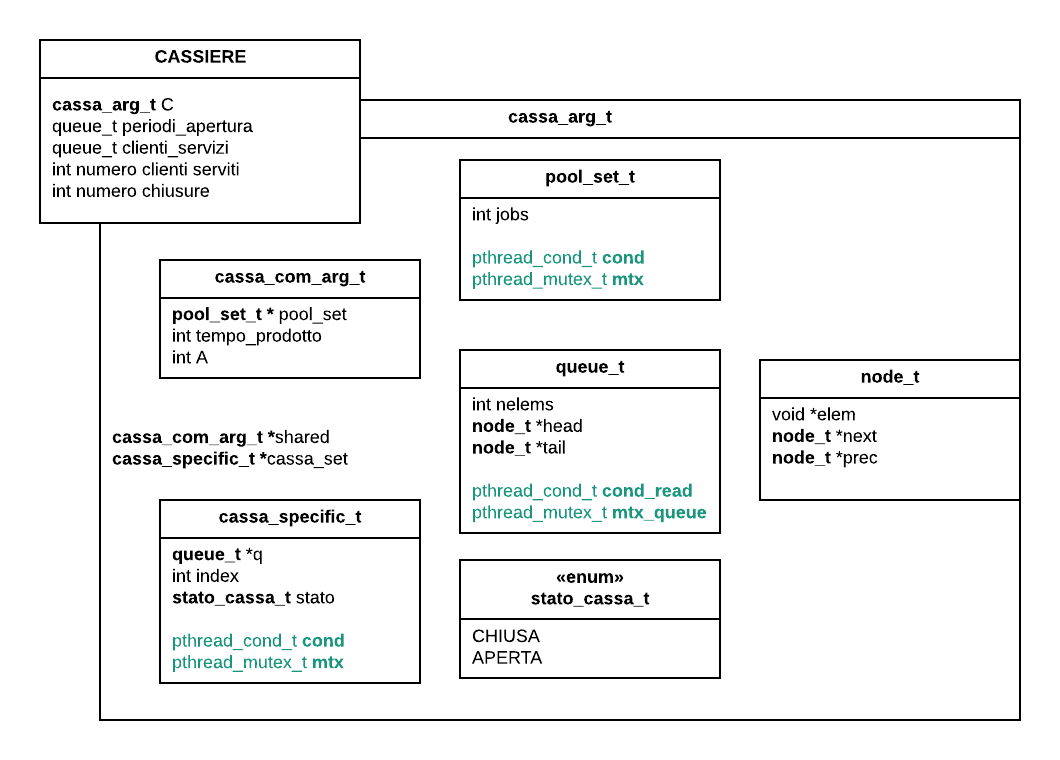
\includegraphics[scale=0.8]{cassa.png}
	\label{fig:cassa}
\end{figure}

\textit{shared} è condiviso fra tutte le casse mentre \textit{cassa\_set} è specifico per ogni cassa
la scelta di  usare un'ulteriore struttura dati è 
per  incapsulamente e riservatezza dei dati 
delle che dovranno essere letti dai clienti 
\subsubsection{Concorrenza}
Nel cassiere le variabili accedute in lettura e scrittura da più thread sono:
\begin{itemize}
\item q
\item stato
\end{itemize}

\section{Utilizzo}
Il makefile presente nel progetto contiene il necessario per compilare e testare il programma, usare:
\begin{itemize}
\item \textbf{make}
\item make \textbf{clean} / \textbf{cleanall} per pulire dai file di lavoro usare clean, per ricompilare l'intero progetto usare cleanall (include l'effetto di clean)
\item make \textbf{test1} \ \textbf{test2}
\end{itemize}
La funzione di cambio cassa dei clienti in coda utilizza in genere molta CPU, è possibile disabilitarla settando DFLAGS = -DNO\_CAMBIO\_CASSA nel makefile.\\
Riguardo il parametro S ho reputato opportuno imporre che debba essere > 10 (millisecondi) per non causare troppo overhead.\\
Per una descrizione dei parametri aggiuntivi (A, J, ...) e del file di configurazione accettato si prega di eseguire \textit{make help}.


\end{document}